% Created by tikzDevice version 0.7.0 on 2014-10-24 15:37:14
% !TEX encoding = UTF-8 Unicode
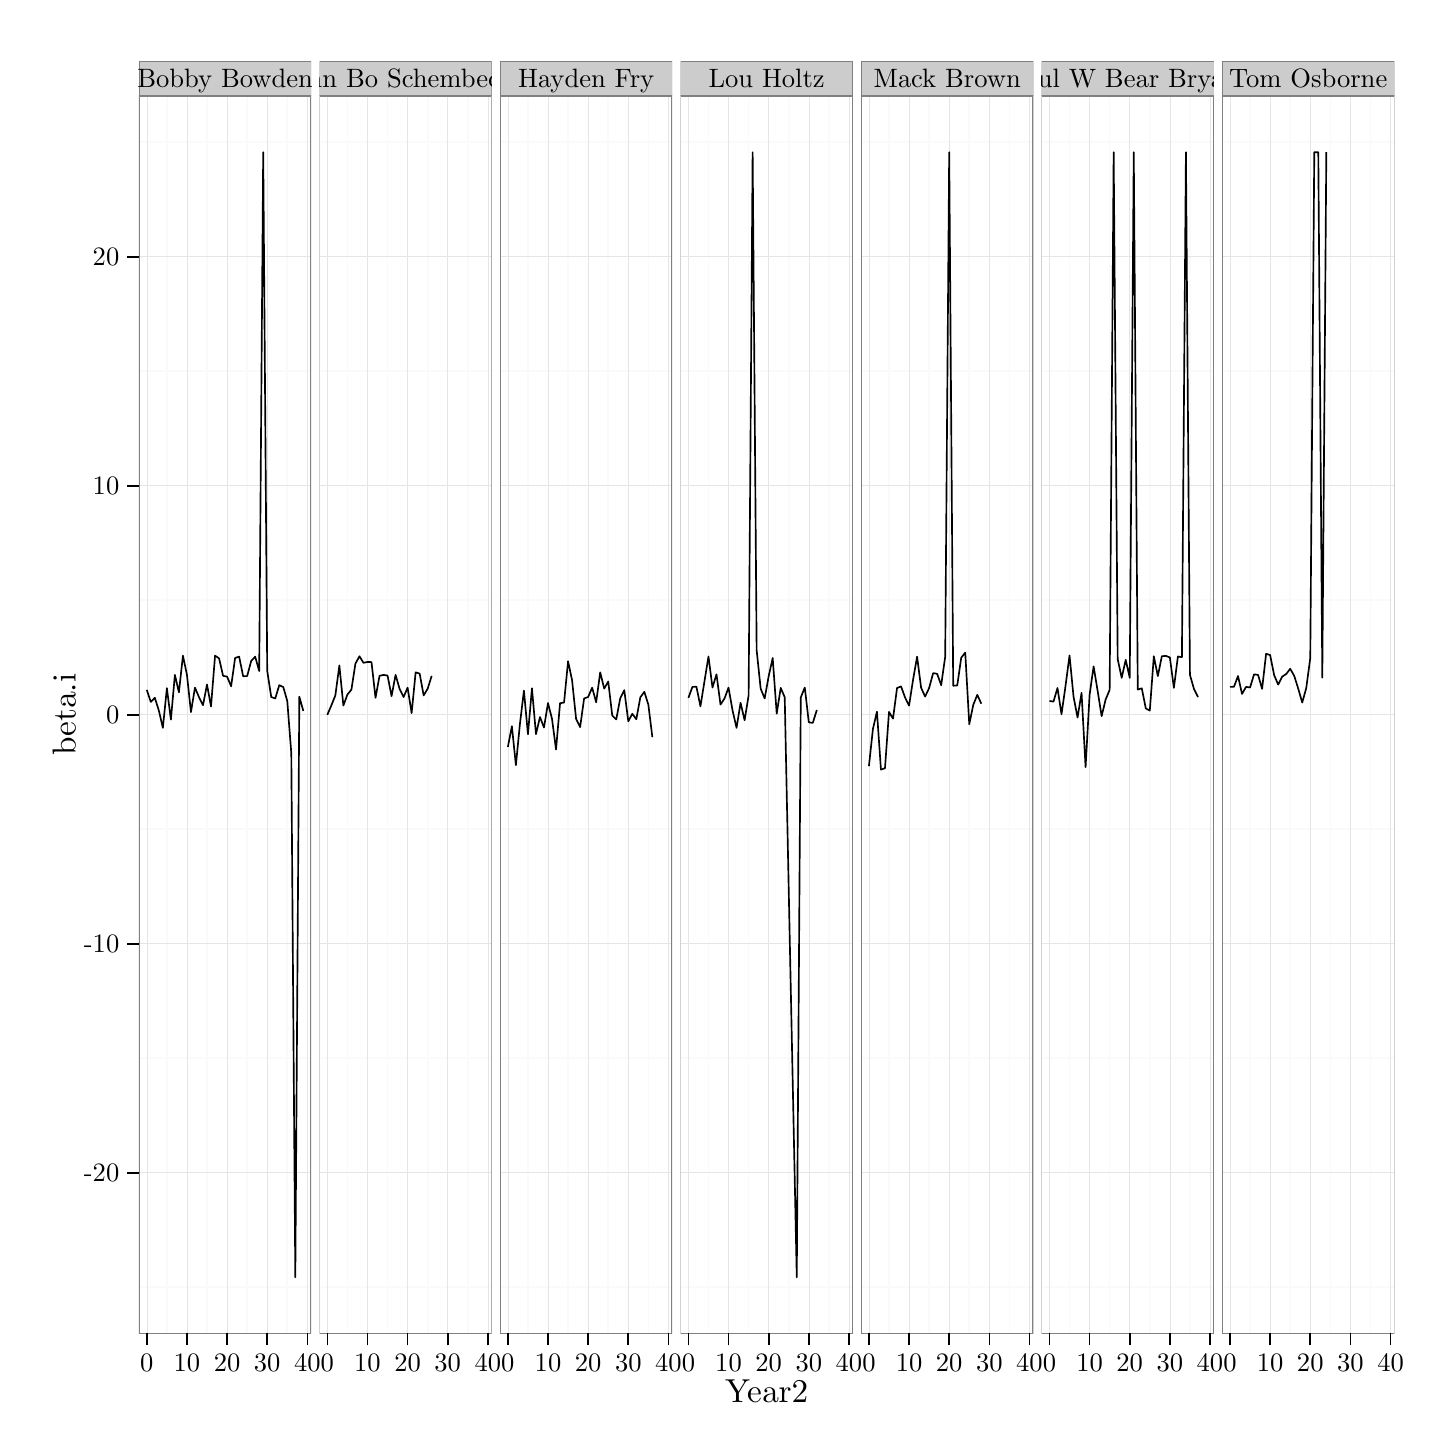
\begin{tikzpicture}[x=1pt,y=1pt]
\definecolor[named]{fillColor}{rgb}{1.00,1.00,1.00}
\path[use as bounding box,fill=fillColor,fill opacity=0.00] (0,0) rectangle (505.89,505.89);
\begin{scope}
\path[clip] (  0.00,  0.00) rectangle (505.89,505.89);
\definecolor[named]{drawColor}{rgb}{1.00,1.00,1.00}
\definecolor[named]{fillColor}{rgb}{1.00,1.00,1.00}

\path[draw=drawColor,line width= 0.6pt,line join=round,line cap=round,fill=fillColor] ( -0.00,  0.00) rectangle (505.89,505.89);
\end{scope}
\begin{scope}
\path[clip] ( 40.22,481.21) rectangle (102.44,493.85);
\definecolor[named]{drawColor}{rgb}{0.50,0.50,0.50}
\definecolor[named]{fillColor}{rgb}{0.80,0.80,0.80}

\path[draw=drawColor,line width= 0.2pt,line join=round,line cap=round,fill=fillColor] ( 40.22,481.21) rectangle (102.44,493.85);
\definecolor[named]{drawColor}{rgb}{0.00,0.00,0.00}

\node[text=drawColor,anchor=base,inner sep=0pt, outer sep=0pt, scale=  0.96] at ( 71.33,484.22) {Bobby Bowden};
\end{scope}
\begin{scope}
\path[clip] (105.45,481.21) rectangle (167.68,493.85);
\definecolor[named]{drawColor}{rgb}{0.50,0.50,0.50}
\definecolor[named]{fillColor}{rgb}{0.80,0.80,0.80}

\path[draw=drawColor,line width= 0.2pt,line join=round,line cap=round,fill=fillColor] (105.45,481.21) rectangle (167.68,493.85);
\definecolor[named]{drawColor}{rgb}{0.00,0.00,0.00}

\node[text=drawColor,anchor=base,inner sep=0pt, outer sep=0pt, scale=  0.96] at (136.56,484.22) {Glenn Bo Schembechler};
\end{scope}
\begin{scope}
\path[clip] (170.69,481.21) rectangle (232.91,493.85);
\definecolor[named]{drawColor}{rgb}{0.50,0.50,0.50}
\definecolor[named]{fillColor}{rgb}{0.80,0.80,0.80}

\path[draw=drawColor,line width= 0.2pt,line join=round,line cap=round,fill=fillColor] (170.69,481.21) rectangle (232.91,493.85);
\definecolor[named]{drawColor}{rgb}{0.00,0.00,0.00}

\node[text=drawColor,anchor=base,inner sep=0pt, outer sep=0pt, scale=  0.96] at (201.80,484.22) {Hayden Fry};
\end{scope}
\begin{scope}
\path[clip] (235.92,481.21) rectangle (298.14,493.85);
\definecolor[named]{drawColor}{rgb}{0.50,0.50,0.50}
\definecolor[named]{fillColor}{rgb}{0.80,0.80,0.80}

\path[draw=drawColor,line width= 0.2pt,line join=round,line cap=round,fill=fillColor] (235.92,481.21) rectangle (298.14,493.85);
\definecolor[named]{drawColor}{rgb}{0.00,0.00,0.00}

\node[text=drawColor,anchor=base,inner sep=0pt, outer sep=0pt, scale=  0.96] at (267.03,484.22) {Lou Holtz};
\end{scope}
\begin{scope}
\path[clip] (301.15,481.21) rectangle (363.38,493.85);
\definecolor[named]{drawColor}{rgb}{0.50,0.50,0.50}
\definecolor[named]{fillColor}{rgb}{0.80,0.80,0.80}

\path[draw=drawColor,line width= 0.2pt,line join=round,line cap=round,fill=fillColor] (301.15,481.21) rectangle (363.38,493.85);
\definecolor[named]{drawColor}{rgb}{0.00,0.00,0.00}

\node[text=drawColor,anchor=base,inner sep=0pt, outer sep=0pt, scale=  0.96] at (332.27,484.22) {Mack Brown};
\end{scope}
\begin{scope}
\path[clip] (366.39,481.21) rectangle (428.61,493.85);
\definecolor[named]{drawColor}{rgb}{0.50,0.50,0.50}
\definecolor[named]{fillColor}{rgb}{0.80,0.80,0.80}

\path[draw=drawColor,line width= 0.2pt,line join=round,line cap=round,fill=fillColor] (366.39,481.21) rectangle (428.61,493.85);
\definecolor[named]{drawColor}{rgb}{0.00,0.00,0.00}

\node[text=drawColor,anchor=base,inner sep=0pt, outer sep=0pt, scale=  0.96] at (397.50,484.22) {Paul W Bear Bryant};
\end{scope}
\begin{scope}
\path[clip] (431.62,481.21) rectangle (493.85,493.85);
\definecolor[named]{drawColor}{rgb}{0.50,0.50,0.50}
\definecolor[named]{fillColor}{rgb}{0.80,0.80,0.80}

\path[draw=drawColor,line width= 0.2pt,line join=round,line cap=round,fill=fillColor] (431.62,481.21) rectangle (493.85,493.85);
\definecolor[named]{drawColor}{rgb}{0.00,0.00,0.00}

\node[text=drawColor,anchor=base,inner sep=0pt, outer sep=0pt, scale=  0.96] at (462.73,484.22) {Tom Osborne};
\end{scope}
\begin{scope}
\path[clip] ( 40.22, 34.03) rectangle (102.44,481.21);
\definecolor[named]{fillColor}{rgb}{1.00,1.00,1.00}

\path[fill=fillColor] ( 40.22, 34.03) rectangle (102.44,481.21);
\definecolor[named]{drawColor}{rgb}{0.98,0.98,0.98}

\path[draw=drawColor,line width= 0.6pt,line join=round] ( 40.22, 50.77) --
	(102.44, 50.77);

\path[draw=drawColor,line width= 0.6pt,line join=round] ( 40.22,133.51) --
	(102.44,133.51);

\path[draw=drawColor,line width= 0.6pt,line join=round] ( 40.22,216.25) --
	(102.44,216.25);

\path[draw=drawColor,line width= 0.6pt,line join=round] ( 40.22,298.99) --
	(102.44,298.99);

\path[draw=drawColor,line width= 0.6pt,line join=round] ( 40.22,381.73) --
	(102.44,381.73);

\path[draw=drawColor,line width= 0.6pt,line join=round] ( 40.22,464.47) --
	(102.44,464.47);

\path[draw=drawColor,line width= 0.6pt,line join=round] ( 50.30, 34.03) --
	( 50.30,481.21);

\path[draw=drawColor,line width= 0.6pt,line join=round] ( 64.80, 34.03) --
	( 64.80,481.21);

\path[draw=drawColor,line width= 0.6pt,line join=round] ( 79.31, 34.03) --
	( 79.31,481.21);

\path[draw=drawColor,line width= 0.6pt,line join=round] ( 93.81, 34.03) --
	( 93.81,481.21);
\definecolor[named]{drawColor}{rgb}{0.90,0.90,0.90}

\path[draw=drawColor,line width= 0.2pt,line join=round] ( 40.22, 92.14) --
	(102.44, 92.14);

\path[draw=drawColor,line width= 0.2pt,line join=round] ( 40.22,174.88) --
	(102.44,174.88);

\path[draw=drawColor,line width= 0.2pt,line join=round] ( 40.22,257.62) --
	(102.44,257.62);

\path[draw=drawColor,line width= 0.2pt,line join=round] ( 40.22,340.36) --
	(102.44,340.36);

\path[draw=drawColor,line width= 0.2pt,line join=round] ( 40.22,423.10) --
	(102.44,423.10);

\path[draw=drawColor,line width= 0.2pt,line join=round] ( 43.05, 34.03) --
	( 43.05,481.21);

\path[draw=drawColor,line width= 0.2pt,line join=round] ( 57.55, 34.03) --
	( 57.55,481.21);

\path[draw=drawColor,line width= 0.2pt,line join=round] ( 72.06, 34.03) --
	( 72.06,481.21);

\path[draw=drawColor,line width= 0.2pt,line join=round] ( 86.56, 34.03) --
	( 86.56,481.21);

\path[draw=drawColor,line width= 0.2pt,line join=round] (101.06, 34.03) --
	(101.06,481.21);
\definecolor[named]{drawColor}{rgb}{0.00,0.00,0.00}

\path[draw=drawColor,line width= 0.6pt,line join=round] ( 43.05,266.59) --
	( 44.50,262.26) --
	( 45.95,263.73) --
	( 47.40,259.12) --
	( 48.85,252.88) --
	( 50.30,267.22) --
	( 51.75,255.85) --
	( 53.20,272.01) --
	( 54.65,265.72) --
	( 56.10,278.96) --
	( 57.55,272.08) --
	( 59.00,258.57) --
	( 60.45,267.42) --
	( 61.90,263.99) --
	( 63.35,261.06) --
	( 64.80,268.52) --
	( 66.25,260.60) --
	( 67.71,278.95) --
	( 69.16,277.98) --
	( 70.61,271.67) --
	( 72.06,271.38) --
	( 73.51,267.92) --
	( 74.96,278.12) --
	( 76.41,278.61) --
	( 77.86,271.54) --
	( 79.31,271.58) --
	( 80.76,277.04) --
	( 82.21,278.59) --
	( 83.66,273.42) --
	( 85.11,460.88) --
	( 86.56,273.47) --
	( 88.01,264.03) --
	( 89.46,263.49) --
	( 90.91,268.29) --
	( 92.36,267.62) --
	( 93.81,262.57) --
	( 95.26,243.73) --
	( 96.71, 54.36) --
	( 98.16,264.15) --
	( 99.61,258.97);
\definecolor[named]{drawColor}{rgb}{0.50,0.50,0.50}

\path[draw=drawColor,line width= 0.6pt,line join=round,line cap=round] ( 40.22, 34.03) rectangle (102.44,481.21);
\end{scope}
\begin{scope}
\path[clip] (105.45, 34.03) rectangle (167.68,481.21);
\definecolor[named]{fillColor}{rgb}{1.00,1.00,1.00}

\path[fill=fillColor] (105.45, 34.03) rectangle (167.68,481.21);
\definecolor[named]{drawColor}{rgb}{0.98,0.98,0.98}

\path[draw=drawColor,line width= 0.6pt,line join=round] (105.45, 50.77) --
	(167.68, 50.77);

\path[draw=drawColor,line width= 0.6pt,line join=round] (105.45,133.51) --
	(167.68,133.51);

\path[draw=drawColor,line width= 0.6pt,line join=round] (105.45,216.25) --
	(167.68,216.25);

\path[draw=drawColor,line width= 0.6pt,line join=round] (105.45,298.99) --
	(167.68,298.99);

\path[draw=drawColor,line width= 0.6pt,line join=round] (105.45,381.73) --
	(167.68,381.73);

\path[draw=drawColor,line width= 0.6pt,line join=round] (105.45,464.47) --
	(167.68,464.47);

\path[draw=drawColor,line width= 0.6pt,line join=round] (115.53, 34.03) --
	(115.53,481.21);

\path[draw=drawColor,line width= 0.6pt,line join=round] (130.04, 34.03) --
	(130.04,481.21);

\path[draw=drawColor,line width= 0.6pt,line join=round] (144.54, 34.03) --
	(144.54,481.21);

\path[draw=drawColor,line width= 0.6pt,line join=round] (159.05, 34.03) --
	(159.05,481.21);
\definecolor[named]{drawColor}{rgb}{0.90,0.90,0.90}

\path[draw=drawColor,line width= 0.2pt,line join=round] (105.45, 92.14) --
	(167.68, 92.14);

\path[draw=drawColor,line width= 0.2pt,line join=round] (105.45,174.88) --
	(167.68,174.88);

\path[draw=drawColor,line width= 0.2pt,line join=round] (105.45,257.62) --
	(167.68,257.62);

\path[draw=drawColor,line width= 0.2pt,line join=round] (105.45,340.36) --
	(167.68,340.36);

\path[draw=drawColor,line width= 0.2pt,line join=round] (105.45,423.10) --
	(167.68,423.10);

\path[draw=drawColor,line width= 0.2pt,line join=round] (108.28, 34.03) --
	(108.28,481.21);

\path[draw=drawColor,line width= 0.2pt,line join=round] (122.79, 34.03) --
	(122.79,481.21);

\path[draw=drawColor,line width= 0.2pt,line join=round] (137.29, 34.03) --
	(137.29,481.21);

\path[draw=drawColor,line width= 0.2pt,line join=round] (151.79, 34.03) --
	(151.79,481.21);

\path[draw=drawColor,line width= 0.2pt,line join=round] (166.30, 34.03) --
	(166.30,481.21);
\definecolor[named]{drawColor}{rgb}{0.00,0.00,0.00}

\path[draw=drawColor,line width= 0.6pt,line join=round] (108.28,257.59) --
	(109.73,260.96) --
	(111.18,264.62) --
	(112.63,275.43) --
	(114.08,260.94) --
	(115.53,264.90) --
	(116.98,266.69) --
	(118.43,276.07) --
	(119.89,278.75) --
	(121.34,276.37) --
	(122.79,276.69) --
	(124.24,276.63) --
	(125.69,263.73) --
	(127.14,271.67) --
	(128.59,272.01) --
	(130.04,271.78) --
	(131.49,264.33) --
	(132.94,272.02) --
	(134.39,266.95) --
	(135.84,264.01) --
	(137.29,267.40) --
	(138.74,258.20) --
	(140.19,272.93) --
	(141.64,272.49) --
	(143.09,264.59) --
	(144.54,267.03) --
	(145.99,271.67);
\definecolor[named]{drawColor}{rgb}{0.50,0.50,0.50}

\path[draw=drawColor,line width= 0.6pt,line join=round,line cap=round] (105.45, 34.03) rectangle (167.68,481.21);
\end{scope}
\begin{scope}
\path[clip] (170.69, 34.03) rectangle (232.91,481.21);
\definecolor[named]{fillColor}{rgb}{1.00,1.00,1.00}

\path[fill=fillColor] (170.69, 34.03) rectangle (232.91,481.21);
\definecolor[named]{drawColor}{rgb}{0.98,0.98,0.98}

\path[draw=drawColor,line width= 0.6pt,line join=round] (170.69, 50.77) --
	(232.91, 50.77);

\path[draw=drawColor,line width= 0.6pt,line join=round] (170.69,133.51) --
	(232.91,133.51);

\path[draw=drawColor,line width= 0.6pt,line join=round] (170.69,216.25) --
	(232.91,216.25);

\path[draw=drawColor,line width= 0.6pt,line join=round] (170.69,298.99) --
	(232.91,298.99);

\path[draw=drawColor,line width= 0.6pt,line join=round] (170.69,381.73) --
	(232.91,381.73);

\path[draw=drawColor,line width= 0.6pt,line join=round] (170.69,464.47) --
	(232.91,464.47);

\path[draw=drawColor,line width= 0.6pt,line join=round] (180.77, 34.03) --
	(180.77,481.21);

\path[draw=drawColor,line width= 0.6pt,line join=round] (195.27, 34.03) --
	(195.27,481.21);

\path[draw=drawColor,line width= 0.6pt,line join=round] (209.78, 34.03) --
	(209.78,481.21);

\path[draw=drawColor,line width= 0.6pt,line join=round] (224.28, 34.03) --
	(224.28,481.21);
\definecolor[named]{drawColor}{rgb}{0.90,0.90,0.90}

\path[draw=drawColor,line width= 0.2pt,line join=round] (170.69, 92.14) --
	(232.91, 92.14);

\path[draw=drawColor,line width= 0.2pt,line join=round] (170.69,174.88) --
	(232.91,174.88);

\path[draw=drawColor,line width= 0.2pt,line join=round] (170.69,257.62) --
	(232.91,257.62);

\path[draw=drawColor,line width= 0.2pt,line join=round] (170.69,340.36) --
	(232.91,340.36);

\path[draw=drawColor,line width= 0.2pt,line join=round] (170.69,423.10) --
	(232.91,423.10);

\path[draw=drawColor,line width= 0.2pt,line join=round] (173.52, 34.03) --
	(173.52,481.21);

\path[draw=drawColor,line width= 0.2pt,line join=round] (188.02, 34.03) --
	(188.02,481.21);

\path[draw=drawColor,line width= 0.2pt,line join=round] (202.52, 34.03) --
	(202.52,481.21);

\path[draw=drawColor,line width= 0.2pt,line join=round] (217.03, 34.03) --
	(217.03,481.21);

\path[draw=drawColor,line width= 0.2pt,line join=round] (231.53, 34.03) --
	(231.53,481.21);
\definecolor[named]{drawColor}{rgb}{0.00,0.00,0.00}

\path[draw=drawColor,line width= 0.6pt,line join=round] (173.52,245.99) --
	(174.97,253.46) --
	(176.42,239.39) --
	(177.87,254.25) --
	(179.32,266.32) --
	(180.77,250.56) --
	(182.22,267.17) --
	(183.67,250.60) --
	(185.12,256.78) --
	(186.57,252.99) --
	(188.02,261.84) --
	(189.47,256.10) --
	(190.92,245.03) --
	(192.37,261.76) --
	(193.82,262.03) --
	(195.27,276.94) --
	(196.72,270.07) --
	(198.17,256.11) --
	(199.62,253.14) --
	(201.07,263.51) --
	(202.52,264.01) --
	(203.97,267.40) --
	(205.42,262.12) --
	(206.88,272.93) --
	(208.33,267.05) --
	(209.78,269.64) --
	(211.23,257.34) --
	(212.68,255.92) --
	(214.13,263.60) --
	(215.58,266.48) --
	(217.03,255.25) --
	(218.48,257.96) --
	(219.93,255.99) --
	(221.38,263.90) --
	(222.83,265.90) --
	(224.28,261.25) --
	(225.73,249.49);
\definecolor[named]{drawColor}{rgb}{0.50,0.50,0.50}

\path[draw=drawColor,line width= 0.6pt,line join=round,line cap=round] (170.69, 34.03) rectangle (232.91,481.21);
\end{scope}
\begin{scope}
\path[clip] (235.92, 34.03) rectangle (298.14,481.21);
\definecolor[named]{fillColor}{rgb}{1.00,1.00,1.00}

\path[fill=fillColor] (235.92, 34.03) rectangle (298.14,481.21);
\definecolor[named]{drawColor}{rgb}{0.98,0.98,0.98}

\path[draw=drawColor,line width= 0.6pt,line join=round] (235.92, 50.77) --
	(298.14, 50.77);

\path[draw=drawColor,line width= 0.6pt,line join=round] (235.92,133.51) --
	(298.14,133.51);

\path[draw=drawColor,line width= 0.6pt,line join=round] (235.92,216.25) --
	(298.14,216.25);

\path[draw=drawColor,line width= 0.6pt,line join=round] (235.92,298.99) --
	(298.14,298.99);

\path[draw=drawColor,line width= 0.6pt,line join=round] (235.92,381.73) --
	(298.14,381.73);

\path[draw=drawColor,line width= 0.6pt,line join=round] (235.92,464.47) --
	(298.14,464.47);

\path[draw=drawColor,line width= 0.6pt,line join=round] (246.00, 34.03) --
	(246.00,481.21);

\path[draw=drawColor,line width= 0.6pt,line join=round] (260.51, 34.03) --
	(260.51,481.21);

\path[draw=drawColor,line width= 0.6pt,line join=round] (275.01, 34.03) --
	(275.01,481.21);

\path[draw=drawColor,line width= 0.6pt,line join=round] (289.51, 34.03) --
	(289.51,481.21);
\definecolor[named]{drawColor}{rgb}{0.90,0.90,0.90}

\path[draw=drawColor,line width= 0.2pt,line join=round] (235.92, 92.14) --
	(298.14, 92.14);

\path[draw=drawColor,line width= 0.2pt,line join=round] (235.92,174.88) --
	(298.14,174.88);

\path[draw=drawColor,line width= 0.2pt,line join=round] (235.92,257.62) --
	(298.14,257.62);

\path[draw=drawColor,line width= 0.2pt,line join=round] (235.92,340.36) --
	(298.14,340.36);

\path[draw=drawColor,line width= 0.2pt,line join=round] (235.92,423.10) --
	(298.14,423.10);

\path[draw=drawColor,line width= 0.2pt,line join=round] (238.75, 34.03) --
	(238.75,481.21);

\path[draw=drawColor,line width= 0.2pt,line join=round] (253.25, 34.03) --
	(253.25,481.21);

\path[draw=drawColor,line width= 0.2pt,line join=round] (267.76, 34.03) --
	(267.76,481.21);

\path[draw=drawColor,line width= 0.2pt,line join=round] (282.26, 34.03) --
	(282.26,481.21);

\path[draw=drawColor,line width= 0.2pt,line join=round] (296.77, 34.03) --
	(296.77,481.21);
\definecolor[named]{drawColor}{rgb}{0.00,0.00,0.00}

\path[draw=drawColor,line width= 0.6pt,line join=round] (238.75,263.73) --
	(240.20,267.67) --
	(241.65,267.73) --
	(243.10,260.65) --
	(246.00,278.66) --
	(247.45,267.46) --
	(248.90,272.21) --
	(250.35,261.28) --
	(251.80,263.51) --
	(253.25,267.42) --
	(254.70,259.19) --
	(256.15,252.87) --
	(257.60,261.93) --
	(259.06,255.63) --
	(260.51,264.59) --
	(261.96,460.88) --
	(263.41,280.98) --
	(264.86,267.05) --
	(266.31,263.51) --
	(267.76,271.54) --
	(269.21,278.10) --
	(270.66,258.02) --
	(272.11,267.30) --
	(273.56,263.92) --
	(277.91, 54.36) --
	(279.36,263.87) --
	(280.81,267.46) --
	(282.26,254.85) --
	(283.71,254.69) --
	(285.16,259.33);
\definecolor[named]{drawColor}{rgb}{0.50,0.50,0.50}

\path[draw=drawColor,line width= 0.6pt,line join=round,line cap=round] (235.92, 34.03) rectangle (298.14,481.21);
\end{scope}
\begin{scope}
\path[clip] (301.15, 34.03) rectangle (363.38,481.21);
\definecolor[named]{fillColor}{rgb}{1.00,1.00,1.00}

\path[fill=fillColor] (301.15, 34.03) rectangle (363.38,481.21);
\definecolor[named]{drawColor}{rgb}{0.98,0.98,0.98}

\path[draw=drawColor,line width= 0.6pt,line join=round] (301.15, 50.77) --
	(363.38, 50.77);

\path[draw=drawColor,line width= 0.6pt,line join=round] (301.15,133.51) --
	(363.38,133.51);

\path[draw=drawColor,line width= 0.6pt,line join=round] (301.15,216.25) --
	(363.38,216.25);

\path[draw=drawColor,line width= 0.6pt,line join=round] (301.15,298.99) --
	(363.38,298.99);

\path[draw=drawColor,line width= 0.6pt,line join=round] (301.15,381.73) --
	(363.38,381.73);

\path[draw=drawColor,line width= 0.6pt,line join=round] (301.15,464.47) --
	(363.38,464.47);

\path[draw=drawColor,line width= 0.6pt,line join=round] (311.24, 34.03) --
	(311.24,481.21);

\path[draw=drawColor,line width= 0.6pt,line join=round] (325.74, 34.03) --
	(325.74,481.21);

\path[draw=drawColor,line width= 0.6pt,line join=round] (340.24, 34.03) --
	(340.24,481.21);

\path[draw=drawColor,line width= 0.6pt,line join=round] (354.75, 34.03) --
	(354.75,481.21);
\definecolor[named]{drawColor}{rgb}{0.90,0.90,0.90}

\path[draw=drawColor,line width= 0.2pt,line join=round] (301.15, 92.14) --
	(363.38, 92.14);

\path[draw=drawColor,line width= 0.2pt,line join=round] (301.15,174.88) --
	(363.38,174.88);

\path[draw=drawColor,line width= 0.2pt,line join=round] (301.15,257.62) --
	(363.38,257.62);

\path[draw=drawColor,line width= 0.2pt,line join=round] (301.15,340.36) --
	(363.38,340.36);

\path[draw=drawColor,line width= 0.2pt,line join=round] (301.15,423.10) --
	(363.38,423.10);

\path[draw=drawColor,line width= 0.2pt,line join=round] (303.98, 34.03) --
	(303.98,481.21);

\path[draw=drawColor,line width= 0.2pt,line join=round] (318.49, 34.03) --
	(318.49,481.21);

\path[draw=drawColor,line width= 0.2pt,line join=round] (332.99, 34.03) --
	(332.99,481.21);

\path[draw=drawColor,line width= 0.2pt,line join=round] (347.50, 34.03) --
	(347.50,481.21);

\path[draw=drawColor,line width= 0.2pt,line join=round] (362.00, 34.03) --
	(362.00,481.21);
\definecolor[named]{drawColor}{rgb}{0.00,0.00,0.00}

\path[draw=drawColor,line width= 0.6pt,line join=round] (303.98,239.03) --
	(305.43,252.48) --
	(306.88,258.72) --
	(308.33,237.80) --
	(309.78,238.26) --
	(311.24,258.63) --
	(312.69,256.22) --
	(314.14,267.27) --
	(315.59,267.85) --
	(317.04,263.85) --
	(318.49,260.91) --
	(319.94,270.31) --
	(321.39,278.59) --
	(322.84,267.36) --
	(324.29,264.18) --
	(325.74,267.28) --
	(327.19,272.66) --
	(328.64,272.40) --
	(330.09,268.29) --
	(331.54,278.54) --
	(332.99,460.88) --
	(334.44,268.10) --
	(335.89,268.18) --
	(337.34,278.23) --
	(338.79,280.07) --
	(340.24,254.16) --
	(341.69,261.20) --
	(343.14,264.81) --
	(344.59,261.60);
\definecolor[named]{drawColor}{rgb}{0.50,0.50,0.50}

\path[draw=drawColor,line width= 0.6pt,line join=round,line cap=round] (301.15, 34.03) rectangle (363.38,481.21);
\end{scope}
\begin{scope}
\path[clip] (366.39, 34.03) rectangle (428.61,481.21);
\definecolor[named]{fillColor}{rgb}{1.00,1.00,1.00}

\path[fill=fillColor] (366.39, 34.03) rectangle (428.61,481.21);
\definecolor[named]{drawColor}{rgb}{0.98,0.98,0.98}

\path[draw=drawColor,line width= 0.6pt,line join=round] (366.39, 50.77) --
	(428.61, 50.77);

\path[draw=drawColor,line width= 0.6pt,line join=round] (366.39,133.51) --
	(428.61,133.51);

\path[draw=drawColor,line width= 0.6pt,line join=round] (366.39,216.25) --
	(428.61,216.25);

\path[draw=drawColor,line width= 0.6pt,line join=round] (366.39,298.99) --
	(428.61,298.99);

\path[draw=drawColor,line width= 0.6pt,line join=round] (366.39,381.73) --
	(428.61,381.73);

\path[draw=drawColor,line width= 0.6pt,line join=round] (366.39,464.47) --
	(428.61,464.47);

\path[draw=drawColor,line width= 0.6pt,line join=round] (376.47, 34.03) --
	(376.47,481.21);

\path[draw=drawColor,line width= 0.6pt,line join=round] (390.97, 34.03) --
	(390.97,481.21);

\path[draw=drawColor,line width= 0.6pt,line join=round] (405.48, 34.03) --
	(405.48,481.21);

\path[draw=drawColor,line width= 0.6pt,line join=round] (419.98, 34.03) --
	(419.98,481.21);
\definecolor[named]{drawColor}{rgb}{0.90,0.90,0.90}

\path[draw=drawColor,line width= 0.2pt,line join=round] (366.39, 92.14) --
	(428.61, 92.14);

\path[draw=drawColor,line width= 0.2pt,line join=round] (366.39,174.88) --
	(428.61,174.88);

\path[draw=drawColor,line width= 0.2pt,line join=round] (366.39,257.62) --
	(428.61,257.62);

\path[draw=drawColor,line width= 0.2pt,line join=round] (366.39,340.36) --
	(428.61,340.36);

\path[draw=drawColor,line width= 0.2pt,line join=round] (366.39,423.10) --
	(428.61,423.10);

\path[draw=drawColor,line width= 0.2pt,line join=round] (369.22, 34.03) --
	(369.22,481.21);

\path[draw=drawColor,line width= 0.2pt,line join=round] (383.72, 34.03) --
	(383.72,481.21);

\path[draw=drawColor,line width= 0.2pt,line join=round] (398.23, 34.03) --
	(398.23,481.21);

\path[draw=drawColor,line width= 0.2pt,line join=round] (412.73, 34.03) --
	(412.73,481.21);

\path[draw=drawColor,line width= 0.2pt,line join=round] (427.23, 34.03) --
	(427.23,481.21);
\definecolor[named]{drawColor}{rgb}{0.00,0.00,0.00}

\path[draw=drawColor,line width= 0.6pt,line join=round] (369.22,262.60) --
	(370.67,262.35) --
	(372.12,267.27) --
	(373.57,257.79) --
	(375.02,268.01) --
	(376.47,279.06) --
	(377.92,264.14) --
	(379.37,256.61) --
	(380.82,265.53) --
	(382.27,238.67) --
	(383.72,264.79) --
	(385.17,275.10) --
	(386.62,266.29) --
	(388.07,257.10) --
	(389.52,263.13) --
	(390.97,266.61) --
	(392.42,460.88) --
	(393.87,277.71) --
	(395.32,270.95) --
	(396.77,277.46) --
	(398.23,270.93) --
	(399.68,460.88) --
	(401.13,266.72) --
	(402.58,267.17) --
	(404.03,259.89) --
	(405.48,259.13) --
	(406.93,278.75) --
	(408.38,271.57) --
	(409.83,278.75) --
	(411.28,278.89) --
	(412.73,278.32) --
	(414.18,267.33) --
	(415.63,278.66) --
	(417.08,278.42) --
	(418.53,460.88) --
	(419.98,272.03) --
	(421.43,266.95) --
	(422.88,264.01);
\definecolor[named]{drawColor}{rgb}{0.50,0.50,0.50}

\path[draw=drawColor,line width= 0.6pt,line join=round,line cap=round] (366.39, 34.03) rectangle (428.61,481.21);
\end{scope}
\begin{scope}
\path[clip] (431.62, 34.03) rectangle (493.85,481.21);
\definecolor[named]{fillColor}{rgb}{1.00,1.00,1.00}

\path[fill=fillColor] (431.62, 34.03) rectangle (493.85,481.21);
\definecolor[named]{drawColor}{rgb}{0.98,0.98,0.98}

\path[draw=drawColor,line width= 0.6pt,line join=round] (431.62, 50.77) --
	(493.85, 50.77);

\path[draw=drawColor,line width= 0.6pt,line join=round] (431.62,133.51) --
	(493.85,133.51);

\path[draw=drawColor,line width= 0.6pt,line join=round] (431.62,216.25) --
	(493.85,216.25);

\path[draw=drawColor,line width= 0.6pt,line join=round] (431.62,298.99) --
	(493.85,298.99);

\path[draw=drawColor,line width= 0.6pt,line join=round] (431.62,381.73) --
	(493.85,381.73);

\path[draw=drawColor,line width= 0.6pt,line join=round] (431.62,464.47) --
	(493.85,464.47);

\path[draw=drawColor,line width= 0.6pt,line join=round] (441.70, 34.03) --
	(441.70,481.21);

\path[draw=drawColor,line width= 0.6pt,line join=round] (456.21, 34.03) --
	(456.21,481.21);

\path[draw=drawColor,line width= 0.6pt,line join=round] (470.71, 34.03) --
	(470.71,481.21);

\path[draw=drawColor,line width= 0.6pt,line join=round] (485.22, 34.03) --
	(485.22,481.21);
\definecolor[named]{drawColor}{rgb}{0.90,0.90,0.90}

\path[draw=drawColor,line width= 0.2pt,line join=round] (431.62, 92.14) --
	(493.85, 92.14);

\path[draw=drawColor,line width= 0.2pt,line join=round] (431.62,174.88) --
	(493.85,174.88);

\path[draw=drawColor,line width= 0.2pt,line join=round] (431.62,257.62) --
	(493.85,257.62);

\path[draw=drawColor,line width= 0.2pt,line join=round] (431.62,340.36) --
	(493.85,340.36);

\path[draw=drawColor,line width= 0.2pt,line join=round] (431.62,423.10) --
	(493.85,423.10);

\path[draw=drawColor,line width= 0.2pt,line join=round] (434.45, 34.03) --
	(434.45,481.21);

\path[draw=drawColor,line width= 0.2pt,line join=round] (448.95, 34.03) --
	(448.95,481.21);

\path[draw=drawColor,line width= 0.2pt,line join=round] (463.46, 34.03) --
	(463.46,481.21);

\path[draw=drawColor,line width= 0.2pt,line join=round] (477.96, 34.03) --
	(477.96,481.21);

\path[draw=drawColor,line width= 0.2pt,line join=round] (492.47, 34.03) --
	(492.47,481.21);
\definecolor[named]{drawColor}{rgb}{0.00,0.00,0.00}

\path[draw=drawColor,line width= 0.6pt,line join=round] (434.45,267.67) --
	(435.90,267.73) --
	(437.35,271.61) --
	(438.80,265.12) --
	(440.25,267.68) --
	(441.70,267.46) --
	(443.15,272.21) --
	(444.60,272.03) --
	(446.05,266.95) --
	(447.50,279.62) --
	(448.95,279.21) --
	(450.41,271.90) --
	(451.86,268.52) --
	(453.31,271.37) --
	(454.76,272.33) --
	(456.21,274.22) --
	(457.66,271.67) --
	(459.11,267.05) --
	(460.56,262.01) --
	(462.01,267.27) --
	(463.46,278.10) --
	(464.91,460.88) --
	(466.36,460.88) --
	(467.81,271.03) --
	(469.26,460.88);
\definecolor[named]{drawColor}{rgb}{0.50,0.50,0.50}

\path[draw=drawColor,line width= 0.6pt,line join=round,line cap=round] (431.62, 34.03) rectangle (493.85,481.21);
\end{scope}
\begin{scope}
\path[clip] (  0.00,  0.00) rectangle (505.89,505.89);
\definecolor[named]{drawColor}{rgb}{0.00,0.00,0.00}

\node[text=drawColor,anchor=base east,inner sep=0pt, outer sep=0pt, scale=  0.96] at ( 33.11, 88.83) {-20};

\node[text=drawColor,anchor=base east,inner sep=0pt, outer sep=0pt, scale=  0.96] at ( 33.11,171.58) {-10};

\node[text=drawColor,anchor=base east,inner sep=0pt, outer sep=0pt, scale=  0.96] at ( 33.11,254.32) {0};

\node[text=drawColor,anchor=base east,inner sep=0pt, outer sep=0pt, scale=  0.96] at ( 33.11,337.06) {10};

\node[text=drawColor,anchor=base east,inner sep=0pt, outer sep=0pt, scale=  0.96] at ( 33.11,419.80) {20};
\end{scope}
\begin{scope}
\path[clip] (  0.00,  0.00) rectangle (505.89,505.89);
\definecolor[named]{drawColor}{rgb}{0.00,0.00,0.00}

\path[draw=drawColor,line width= 0.6pt,line join=round] ( 35.95, 92.14) --
	( 40.22, 92.14);

\path[draw=drawColor,line width= 0.6pt,line join=round] ( 35.95,174.88) --
	( 40.22,174.88);

\path[draw=drawColor,line width= 0.6pt,line join=round] ( 35.95,257.62) --
	( 40.22,257.62);

\path[draw=drawColor,line width= 0.6pt,line join=round] ( 35.95,340.36) --
	( 40.22,340.36);

\path[draw=drawColor,line width= 0.6pt,line join=round] ( 35.95,423.10) --
	( 40.22,423.10);
\end{scope}
\begin{scope}
\path[clip] (  0.00,  0.00) rectangle (505.89,505.89);
\definecolor[named]{drawColor}{rgb}{0.00,0.00,0.00}

\path[draw=drawColor,line width= 0.6pt,line join=round] ( 43.05, 29.77) --
	( 43.05, 34.03);

\path[draw=drawColor,line width= 0.6pt,line join=round] ( 57.55, 29.77) --
	( 57.55, 34.03);

\path[draw=drawColor,line width= 0.6pt,line join=round] ( 72.06, 29.77) --
	( 72.06, 34.03);

\path[draw=drawColor,line width= 0.6pt,line join=round] ( 86.56, 29.77) --
	( 86.56, 34.03);

\path[draw=drawColor,line width= 0.6pt,line join=round] (101.06, 29.77) --
	(101.06, 34.03);
\end{scope}
\begin{scope}
\path[clip] (  0.00,  0.00) rectangle (505.89,505.89);
\definecolor[named]{drawColor}{rgb}{0.00,0.00,0.00}

\node[text=drawColor,anchor=base,inner sep=0pt, outer sep=0pt, scale=  0.96] at ( 43.05, 20.31) {0};

\node[text=drawColor,anchor=base,inner sep=0pt, outer sep=0pt, scale=  0.96] at ( 57.55, 20.31) {10};

\node[text=drawColor,anchor=base,inner sep=0pt, outer sep=0pt, scale=  0.96] at ( 72.06, 20.31) {20};

\node[text=drawColor,anchor=base,inner sep=0pt, outer sep=0pt, scale=  0.96] at ( 86.56, 20.31) {30};

\node[text=drawColor,anchor=base,inner sep=0pt, outer sep=0pt, scale=  0.96] at (101.06, 20.31) {40};
\end{scope}
\begin{scope}
\path[clip] (  0.00,  0.00) rectangle (505.89,505.89);
\definecolor[named]{drawColor}{rgb}{0.00,0.00,0.00}

\path[draw=drawColor,line width= 0.6pt,line join=round] (108.28, 29.77) --
	(108.28, 34.03);

\path[draw=drawColor,line width= 0.6pt,line join=round] (122.79, 29.77) --
	(122.79, 34.03);

\path[draw=drawColor,line width= 0.6pt,line join=round] (137.29, 29.77) --
	(137.29, 34.03);

\path[draw=drawColor,line width= 0.6pt,line join=round] (151.79, 29.77) --
	(151.79, 34.03);

\path[draw=drawColor,line width= 0.6pt,line join=round] (166.30, 29.77) --
	(166.30, 34.03);
\end{scope}
\begin{scope}
\path[clip] (  0.00,  0.00) rectangle (505.89,505.89);
\definecolor[named]{drawColor}{rgb}{0.00,0.00,0.00}

\node[text=drawColor,anchor=base,inner sep=0pt, outer sep=0pt, scale=  0.96] at (108.28, 20.31) {0};

\node[text=drawColor,anchor=base,inner sep=0pt, outer sep=0pt, scale=  0.96] at (122.79, 20.31) {10};

\node[text=drawColor,anchor=base,inner sep=0pt, outer sep=0pt, scale=  0.96] at (137.29, 20.31) {20};

\node[text=drawColor,anchor=base,inner sep=0pt, outer sep=0pt, scale=  0.96] at (151.79, 20.31) {30};

\node[text=drawColor,anchor=base,inner sep=0pt, outer sep=0pt, scale=  0.96] at (166.30, 20.31) {40};
\end{scope}
\begin{scope}
\path[clip] (  0.00,  0.00) rectangle (505.89,505.89);
\definecolor[named]{drawColor}{rgb}{0.00,0.00,0.00}

\path[draw=drawColor,line width= 0.6pt,line join=round] (173.52, 29.77) --
	(173.52, 34.03);

\path[draw=drawColor,line width= 0.6pt,line join=round] (188.02, 29.77) --
	(188.02, 34.03);

\path[draw=drawColor,line width= 0.6pt,line join=round] (202.52, 29.77) --
	(202.52, 34.03);

\path[draw=drawColor,line width= 0.6pt,line join=round] (217.03, 29.77) --
	(217.03, 34.03);

\path[draw=drawColor,line width= 0.6pt,line join=round] (231.53, 29.77) --
	(231.53, 34.03);
\end{scope}
\begin{scope}
\path[clip] (  0.00,  0.00) rectangle (505.89,505.89);
\definecolor[named]{drawColor}{rgb}{0.00,0.00,0.00}

\node[text=drawColor,anchor=base,inner sep=0pt, outer sep=0pt, scale=  0.96] at (173.52, 20.31) {0};

\node[text=drawColor,anchor=base,inner sep=0pt, outer sep=0pt, scale=  0.96] at (188.02, 20.31) {10};

\node[text=drawColor,anchor=base,inner sep=0pt, outer sep=0pt, scale=  0.96] at (202.52, 20.31) {20};

\node[text=drawColor,anchor=base,inner sep=0pt, outer sep=0pt, scale=  0.96] at (217.03, 20.31) {30};

\node[text=drawColor,anchor=base,inner sep=0pt, outer sep=0pt, scale=  0.96] at (231.53, 20.31) {40};
\end{scope}
\begin{scope}
\path[clip] (  0.00,  0.00) rectangle (505.89,505.89);
\definecolor[named]{drawColor}{rgb}{0.00,0.00,0.00}

\path[draw=drawColor,line width= 0.6pt,line join=round] (238.75, 29.77) --
	(238.75, 34.03);

\path[draw=drawColor,line width= 0.6pt,line join=round] (253.25, 29.77) --
	(253.25, 34.03);

\path[draw=drawColor,line width= 0.6pt,line join=round] (267.76, 29.77) --
	(267.76, 34.03);

\path[draw=drawColor,line width= 0.6pt,line join=round] (282.26, 29.77) --
	(282.26, 34.03);

\path[draw=drawColor,line width= 0.6pt,line join=round] (296.77, 29.77) --
	(296.77, 34.03);
\end{scope}
\begin{scope}
\path[clip] (  0.00,  0.00) rectangle (505.89,505.89);
\definecolor[named]{drawColor}{rgb}{0.00,0.00,0.00}

\node[text=drawColor,anchor=base,inner sep=0pt, outer sep=0pt, scale=  0.96] at (238.75, 20.31) {0};

\node[text=drawColor,anchor=base,inner sep=0pt, outer sep=0pt, scale=  0.96] at (253.25, 20.31) {10};

\node[text=drawColor,anchor=base,inner sep=0pt, outer sep=0pt, scale=  0.96] at (267.76, 20.31) {20};

\node[text=drawColor,anchor=base,inner sep=0pt, outer sep=0pt, scale=  0.96] at (282.26, 20.31) {30};

\node[text=drawColor,anchor=base,inner sep=0pt, outer sep=0pt, scale=  0.96] at (296.77, 20.31) {40};
\end{scope}
\begin{scope}
\path[clip] (  0.00,  0.00) rectangle (505.89,505.89);
\definecolor[named]{drawColor}{rgb}{0.00,0.00,0.00}

\path[draw=drawColor,line width= 0.6pt,line join=round] (303.98, 29.77) --
	(303.98, 34.03);

\path[draw=drawColor,line width= 0.6pt,line join=round] (318.49, 29.77) --
	(318.49, 34.03);

\path[draw=drawColor,line width= 0.6pt,line join=round] (332.99, 29.77) --
	(332.99, 34.03);

\path[draw=drawColor,line width= 0.6pt,line join=round] (347.50, 29.77) --
	(347.50, 34.03);

\path[draw=drawColor,line width= 0.6pt,line join=round] (362.00, 29.77) --
	(362.00, 34.03);
\end{scope}
\begin{scope}
\path[clip] (  0.00,  0.00) rectangle (505.89,505.89);
\definecolor[named]{drawColor}{rgb}{0.00,0.00,0.00}

\node[text=drawColor,anchor=base,inner sep=0pt, outer sep=0pt, scale=  0.96] at (303.98, 20.31) {0};

\node[text=drawColor,anchor=base,inner sep=0pt, outer sep=0pt, scale=  0.96] at (318.49, 20.31) {10};

\node[text=drawColor,anchor=base,inner sep=0pt, outer sep=0pt, scale=  0.96] at (332.99, 20.31) {20};

\node[text=drawColor,anchor=base,inner sep=0pt, outer sep=0pt, scale=  0.96] at (347.50, 20.31) {30};

\node[text=drawColor,anchor=base,inner sep=0pt, outer sep=0pt, scale=  0.96] at (362.00, 20.31) {40};
\end{scope}
\begin{scope}
\path[clip] (  0.00,  0.00) rectangle (505.89,505.89);
\definecolor[named]{drawColor}{rgb}{0.00,0.00,0.00}

\path[draw=drawColor,line width= 0.6pt,line join=round] (369.22, 29.77) --
	(369.22, 34.03);

\path[draw=drawColor,line width= 0.6pt,line join=round] (383.72, 29.77) --
	(383.72, 34.03);

\path[draw=drawColor,line width= 0.6pt,line join=round] (398.23, 29.77) --
	(398.23, 34.03);

\path[draw=drawColor,line width= 0.6pt,line join=round] (412.73, 29.77) --
	(412.73, 34.03);

\path[draw=drawColor,line width= 0.6pt,line join=round] (427.23, 29.77) --
	(427.23, 34.03);
\end{scope}
\begin{scope}
\path[clip] (  0.00,  0.00) rectangle (505.89,505.89);
\definecolor[named]{drawColor}{rgb}{0.00,0.00,0.00}

\node[text=drawColor,anchor=base,inner sep=0pt, outer sep=0pt, scale=  0.96] at (369.22, 20.31) {0};

\node[text=drawColor,anchor=base,inner sep=0pt, outer sep=0pt, scale=  0.96] at (383.72, 20.31) {10};

\node[text=drawColor,anchor=base,inner sep=0pt, outer sep=0pt, scale=  0.96] at (398.23, 20.31) {20};

\node[text=drawColor,anchor=base,inner sep=0pt, outer sep=0pt, scale=  0.96] at (412.73, 20.31) {30};

\node[text=drawColor,anchor=base,inner sep=0pt, outer sep=0pt, scale=  0.96] at (427.23, 20.31) {40};
\end{scope}
\begin{scope}
\path[clip] (  0.00,  0.00) rectangle (505.89,505.89);
\definecolor[named]{drawColor}{rgb}{0.00,0.00,0.00}

\path[draw=drawColor,line width= 0.6pt,line join=round] (434.45, 29.77) --
	(434.45, 34.03);

\path[draw=drawColor,line width= 0.6pt,line join=round] (448.95, 29.77) --
	(448.95, 34.03);

\path[draw=drawColor,line width= 0.6pt,line join=round] (463.46, 29.77) --
	(463.46, 34.03);

\path[draw=drawColor,line width= 0.6pt,line join=round] (477.96, 29.77) --
	(477.96, 34.03);

\path[draw=drawColor,line width= 0.6pt,line join=round] (492.47, 29.77) --
	(492.47, 34.03);
\end{scope}
\begin{scope}
\path[clip] (  0.00,  0.00) rectangle (505.89,505.89);
\definecolor[named]{drawColor}{rgb}{0.00,0.00,0.00}

\node[text=drawColor,anchor=base,inner sep=0pt, outer sep=0pt, scale=  0.96] at (434.45, 20.31) {0};

\node[text=drawColor,anchor=base,inner sep=0pt, outer sep=0pt, scale=  0.96] at (448.95, 20.31) {10};

\node[text=drawColor,anchor=base,inner sep=0pt, outer sep=0pt, scale=  0.96] at (463.46, 20.31) {20};

\node[text=drawColor,anchor=base,inner sep=0pt, outer sep=0pt, scale=  0.96] at (477.96, 20.31) {30};

\node[text=drawColor,anchor=base,inner sep=0pt, outer sep=0pt, scale=  0.96] at (492.47, 20.31) {40};
\end{scope}
\begin{scope}
\path[clip] (  0.00,  0.00) rectangle (505.89,505.89);
\definecolor[named]{drawColor}{rgb}{0.00,0.00,0.00}

\node[text=drawColor,anchor=base,inner sep=0pt, outer sep=0pt, scale=  1.20] at (267.03,  9.03) {Year2};
\end{scope}
\begin{scope}
\path[clip] (  0.00,  0.00) rectangle (505.89,505.89);
\definecolor[named]{drawColor}{rgb}{0.00,0.00,0.00}

\node[text=drawColor,rotate= 90.00,anchor=base,inner sep=0pt, outer sep=0pt, scale=  1.20] at ( 17.30,257.62) {beta.i};
\end{scope}
\end{tikzpicture}
